\documentclass[11pt]{article}

\usepackage[margin=1in]{geometry}
\usepackage{amsmath,amssymb,amsthm}
\usepackage{booktabs}
\usepackage{enumitem}
\usepackage{graphicx}
\usepackage{hyperref}
\usepackage{microtype}
\usepackage{parskip}
\usepackage{placeins}
\usepackage{float}
\usepackage[font=small,labelfont=bf]{caption}
\usepackage{tikz}
\usepackage{pgfplots}
\pgfplotsset{compat=1.18}
\usetikzlibrary{arrows.meta}

\hypersetup{
  colorlinks=true,
  linkcolor=blue,
  citecolor=blue,
  urlcolor=blue
}
\setlength{\emergencystretch}{3em}
\allowdisplaybreaks

\definecolor{figblue}{HTML}{2A6FB0}
\definecolor{figorange}{HTML}{D1622B}
\definecolor{figteal}{HTML}{1D9E75}
\definecolor{figpurple}{HTML}{534AB7}
\definecolor{figink}{HTML}{242424}
\definecolor{figboxgray}{HTML}{A0A0A0}
\definecolor{figlightgray}{HTML}{E8E8E8}
\definecolor{figpaleteal}{HTML}{E8F4F0}
\definecolor{figpalepurple}{HTML}{F1EEFB}

\pgfplotsset{
  every axis/.append style={
    line width=0.5pt,
    axis line style={black!70},
    tick style={line width=0.4pt, black!60},
    label style={font=\small},
    tick label style={font=\footnotesize},
    legend style={font=\footnotesize, draw=none, fill=none},
  },
}

\newtheorem{theorem}{Theorem}[section]
\newtheorem{proposition}[theorem]{Proposition}
\newtheorem{lemma}[theorem]{Lemma}
\newtheorem{corollary}[theorem]{Corollary}
\newtheorem{definition}[theorem]{Definition}

\newcommand{\val}{\operatorname{val}}
\newcommand{\gap}{\operatorname{gap}}
\newcommand{\tol}{\tau_0}

\title{An Exact Approach to Solving the Drop the Handkerchief Game}
\author{James Cenawood\thanks{Code and instructions to reproduce the results
are available in the project repository.}}
\date{July 31, 2026}

\begin{document}
\maketitle

\begin{abstract}
Drop the Handkerchief (DTH) is a death game played during the final arc
''Surpassing The Leader'' of the manga \textit{Usogui} by Toshio Sako.
It is a fully observed, two-player, simultaneous action, zero-sum stochastic game.
Owing to its deadly nature, we solve the complete 60-action timing model under
the frozen survival law of Section~\ref{sec:game}. Once
a player can no longer survive an injection, the game never reads their
cumulative time dead (TTD) again. Quotienting by that observation collapses the
$5.27\times10^{9}$-state transition-closed domain down to $289{,}374{,}121$
equivalence classes (a factor of $18.2$). A potential function organizes those classes
into $1{,}201$ layers and permits one backward sweep over the finite DAG.
Every local value is accepted with a mixed-strategy gap of at most $10^{-6}$
against its full $60\times60$ stage matrix. At the initial state,
$V=0.08985\pm0.00061$, so the first Dropper wins with probability
$0.54493\pm0.00031$ under optimal play. No unilateral change to the selected
policy can improve win probability by more than $6.005\times10^{-4}$.
The largest continuous run covered
$98.1\%$ of the table in $5{,}432$ seconds on one twelve-core desktop.
\end{abstract}

\section{Introduction}
DTH is the pure timing core of the Surpassing the Leader arc wager in
\emph{Usogui}. Two players alternate as \emph{Dropper} and \emph{Checker}.
Each round, both choose a second in $\{1,\dots,60\}$. A successful check adds
the inclusive delay to the Checker's squandered time (ST), then swaps the
roles. A failed check injects that ST plus sixty seconds. Revival follows the
fixed law in Figure~\ref{fig:revival}; otherwise the Checker loses.

The game is finite but large, and each round may require randomization. The
solution follows four steps:

\begin{enumerate}[leftmargin=*]
\item quotient profiles once failure is certainly fatal
  (Section~\ref{sec:quotient});
\item rank every continuing transition with an increasing potential
  (Section~\ref{sec:potential});
\item solve each $60\times60$ stage game and retain a gap certificate
  (Section~\ref{sec:certified});
\item use the matrix's $61$ transition values to avoid scanning all
  $3{,}600$ cells when testing pure play (Section~\ref{sec:stage}).
\end{enumerate}

Section~\ref{sec:computation} reports the computation and its result.
Section~\ref{sec:claims} states what is and is not established.

\subsection*{The key game theory object}

A state keeps exactly the past that can still affect play. At a state $x$,
each player chooses a probability distribution over the sixty seconds:
\[
\Delta_{60}=\left\{\sigma\in\mathbb R^{60}:\sigma_i\ge0,
\ \sum_{i=1}^{60}\sigma_i=1\right\}.
\]
These distributions are mixed strategies. The stage matrix $M(x)$ gives the
payoff for each action pair, so
\[
V(x)=\max_{\sigma_d\in\Delta_{60}}\min_{\sigma_c\in\Delta_{60}}
\sigma_d^{\mathsf T}M(x)\sigma_c.
\]
The matrix entries contain either a terminal payoff or the value of a later
state. This is Bellman recursion. Once transitions are ordered as a DAG,
later values can be substituted backward. Finally,
$V=P(\mathrm{win})-P(\mathrm{loss})=2P(\mathrm{win})-1$, hence
$P(\mathrm{win})=(1+V)/2$.

\section{The game}\label{sec:game}

\begin{definition}[State]\label{def:state}
A player's \emph{profile} is $z=(s,t)$: their current ST and TTD. A live state
is the ordered pair $x=(z_c,z_d)=(s_c,t_c,s_d,t_d)$, written from the
perspective of the current \emph{Dropper}. Here
$s_c,s_d\in\{0,\dots,299\}$ and $t_c,t_d\in\{0,\dots,300\}$.
Terminal payoffs are $+1$ when the current Dropper wins and $-1$ when they
lose.
\end{definition}

\begin{definition}[Actions and timing]\label{def:actions}
Both players simultaneously choose seconds $d,c\in\{1,\dots,60\}$ (drop and
check). The check \emph{succeeds} iff $d\le c$, and then the Checker's ST
grows by the inclusive interval $\ell=c-d+1\in\{1,\dots,60\}$; equal seconds
cost one second, not zero. If $s_c+\ell\ge300$ the cylinder overflows and
the checker dies: the transition ends with payoff $+1$ for the Dropper.
Overflow is uniformly fatal: a cylinder at capacity leaves no revival
headroom for any dose. Otherwise play continues from
\[
(s_c,t_c,s_d,t_d)\ \xrightarrow{\ \text{success, lag }\ell\ }\
(s_d,\,t_d,\,s_c+\ell,\,t_c),
\]
with the roles swapped (the previous Checker drops next).
\end{definition}

For example, $d=12$ and $c=15$ gives a successful check with
$\ell=15-12+1=4$. If instead $c=10$, the check fails and the Checker receives
their accumulated ST plus sixty seconds.

\begin{definition}[Failure, dose, and revival]\label{def:failure}
On a failed check ($d>c$) the checker is injected with the dose
$q=s_c+60$. Survival is possible iff
\begin{equation}\label{eq:survive}
q<300\ \wedge\ q+t_c\le300
\qquad\Longleftrightarrow\qquad
s_c\le239\ \wedge\ s_c+t_c\le240,
\end{equation}
Equality at $q+t_c=300$ remains revival-eligible.
A profile is \emph{revival-eligible} when \eqref{eq:survive} holds and
\emph{failure-fatal} otherwise. These terms describe the next failed check;
both players are still alive in a live state. When the profile is
revival-eligible, the checker revives with probability
\begin{equation}\label{eq:revival}
p(s_c,t_c)\;=\;0.95\left(1-\frac{s_c}{240}\right)0.75^{\,t_c/60},
\end{equation}
their cylinder resets, and their TTD grows by the dose:
\[
(s_c,t_c,s_d,t_d)\ \xrightarrow{\ \text{failure, revive}\ }\
(s_d,\,t_d,\,0,\,t_c+s_c+60)
\quad\text{with probability }p(s_c,t_c),
\]
else the transition ends with payoff $+1$. When \eqref{eq:survive} fails, the
injection is fatal with certainty and $p(s_c,t_c)\equiv0$.
\end{definition}

The source gives no numerical revival odds, but it fixes the qualitative
geometry: a failed check injects the vial contents plus sixty seconds against a
five-minute cap and cumulative deaths/TTD lower revival prospects enough to change
strategy~\cite{stlevidence}. These facts motivate the separable form in
\eqref{eq:revival}. Since $q=s+60$, the acute factor
$1-s/240=(300-q)/240$ is the simplest monotone path from a bare injection to
the lethal dose, so each second of ST consumes an equal share of acute
headroom. TTD records damage carried through earlier revivals;
$0.75^{t/60}$ makes each additional death-minute retain a fixed fraction of
the chance remaining after the acute dose. The source supports the signs and
endpoint, not linearity, multiplicative separation, or the constants $0.95$
and $0.75$; those are explicit modeling choices.

A deliberately coarse sensitivity check varies the baseline alone. The
six-action abstraction measures time in ten-second units, so actions
$1,\dots,6$ represent seconds $10,20,\dots,60$. Four exact solves at baselines
$0.85,0.90,0.95,$ and $0.99$ place the root value between $0.09639$ and
$0.09921$, a span of $0.0028$, while the Dropper's first-action mass moves
from $0.387$ to $0.257$. The value is therefore fairly stable to this one
parameter at coarse resolution, but the policy is not. This check does not
calibrate the TTD factor $0.75$, test multiplicative separation, or establish
full-resolution robustness.

Values are from the current Dropper's perspective and negate when the roles
swap.

\begin{figure}[t]
\centering
\includegraphics[width=0.95\textwidth]{build/figures/seaborn/fig1_revival_probability.pdf}
\caption{The frozen revival law \eqref{eq:revival}. Color and height both
encode probability. The blue edge isolates the linear loss from ST; the
purple edge isolates the exponential loss from TTD. The pale plateau is the
zero-probability region containing $(240,240)$. The orange curtain
marks $s+t=240$: probability is positive on the curtain, except at its
$s=240$ endpoint, and drops to zero immediately beyond it.}
\label{fig:revival}
\end{figure}

\section{Finiteness and stage structure}\label{sec:stage}

\begin{lemma}[Damage strictly increases]\label{lem:damage}
Let $R(x)=s_c+t_c+s_d+t_d$. Every live transition strictly increases $R$:
a successful lag $\ell$ adds $\ell\ge1$, and a revived failure adds exactly
$60$ (the dose $s_c+60$ enters TTD while the ST $s_c$ resets).
\end{lemma}

\begin{corollary}[The game is finite]\label{cor:finite}
$R\le299+300+299+300=1198$ on live states, so every play reaches a terminal
outcome within $1199$ transitions. The game therefore has a unique
value $V(x)\in[-1,1]$ at every live state, obtained by backward induction over the finite
directed acyclic transition graph~\cite{zermelo1913}, solving at each state the
zero-sum simultaneous stage game by von Neumann's minimax
theorem~\cite{vonneumann1928}; the construction is the finite, absorbing
case of a Shapley stochastic game~\cite{shapley1953}.
\end{corollary}

Mixed strategies matter even in a two-action game. In
\[
\begin{pmatrix}1&-1\\-1&1\end{pmatrix},
\]
either fixed row can be punished by a column giving $-1$, while choosing each
row with probability $1/2$ guarantees $0$. DTH uses the same idea with sixty
actions and state-dependent entries.

\begin{proposition}[The 61 transition classes]\label{prop:classes}
Fix a live state $x$ and let $V$ assign values to its children. Write the
Dropper's continuation payoff after a success of lag $\ell$ or a failure as
\begin{align*}
S_\ell&=
\begin{cases}
+1,& s_c+\ell\ge300,\\
-V(s_d,t_d,s_c+\ell,t_c),&\text{else},
\end{cases}\\[3pt]
F&=
\begin{cases}
+1,& (s_c,t_c)\ \text{failure-fatal},\\
p\,\bigl(-V(s_d,t_d,0,t_c+s_c+60)\bigr)+(1-p),&\text{else}.
\end{cases}
\end{align*}
Then the $60\times60$ stage matrix of $x$, with the Dropper as row player, is
\begin{equation}\label{eq:toeplitz}
M(x)_{d,c}=
\begin{cases}
S_{c-d+1}, & c\ge d,\\
F, & c<d,
\end{cases}
\end{equation}
and $V(x)=\val(M(x))$. In particular $M(x)$ carries at most $61$ distinct
entries: it is Toeplitz on and above the diagonal and constant below it.
\end{proposition}

\begin{proof}
A successful cell depends on the actions only through the lag
$\ell=c-d+1$, and every failed cell has the identical transition
distribution; the entries are the expected continuation values, negated for
the role swap. The Bellman equation is Corollary~\ref{cor:finite}.
\end{proof}

\begin{lemma}[$O(60)$ saddle reductions]\label{lem:toeplitz}
Row $d$ of \eqref{eq:toeplitz} contains exactly the prefix
$S_1,\dots,S_{61-d}$ together with $F$ when $d>1$, and column $c$ contains
the prefix $S_1,\dots,S_c$ together with $F$ when $c<60$. Hence with
prefix scans $m_j=\min_{i\le j}S_i$ and $M_j=\max_{i\le j}S_i$,
\begin{align*}
\max_d\min_c M(x)_{d,c}
&=\max_d
\begin{cases}
m_{60}, & d=1,\\
\min(m_{61-d},F), & d>1,
\end{cases}\\[3pt]
\min_c\max_d M(x)_{d,c}
&=\min_c
\begin{cases}
\max(M_{c},F), & c<60,\\
M_{60}, & c=60,
\end{cases}
\end{align*}
computable in $O(60)$ operations, exactly (min and max select one of their
arguments, so the scans introduce no rounding), from the $61$ class values
alone.
\end{lemma}

Figure~\ref{fig:toeplitz} draws the layout. Each row contains a prefix of the
$S$ array, never an arbitrary subset. Two linear scans therefore
reproduce every row minimum and column maximum without materializing the
matrix.

\begin{figure}[t]
\centering
\includegraphics[width=0.98\textwidth]{build/figures/seaborn/fig2_toeplitz_structure.pdf}
\caption{An $8\times8$ view of the stage matrix \eqref{eq:toeplitz}. The lag
$\ell=c-d+1$ is constant on diagonals, while every failed check has value
$F$. Row minima and column maxima reduce to prefix scans
(Lemma~\ref{lem:toeplitz}), giving the same result as a scan of all
$3{,}600$ cells.}
\label{fig:toeplitz}
\end{figure}

\section{The failure-fatal quotient}\label{sec:quotient}

The model reads a player's TTD only in the revival probability
\eqref{eq:revival}. Once failure is certainly fatal, the exact TTD has no
remaining effect.

For example, profiles $(250,60)$ and $(250,300)$ both receive dose $310$ on a
failed check, so failure is fatal in either case. Success only raises ST and
cannot restore revival. Their TTDs can therefore share the sentinel
$(250,\bot)$.

\begin{lemma}[Failure-fatality is absorbing]\label{lem:absorbing}
If the profile $(s,t)$ is failure-fatal, then $(s',t)$ is failure-fatal for every
$s'\ge s$. Since a successful check raises a player's ST and leaves their
TTD unchanged, and a failed check either ends the game for them or requires
\eqref{eq:survive}, no continuing transition can make the profile
revival-eligible again.
\end{lemma}

\begin{theorem}[Quotient soundness]\label{thm:quotient}
Define $\varphi(s,t)=(s,t)$ when $(s,t)$ is revival-eligible and
$\varphi(s,t)=(s,\bot)$ otherwise. Apply this map to each player's profile
independently. Then any two
live states with equal images under $\varphi$
have identical stage matrices up to $\varphi$-identification of their
children, and hence identical values: $V$ factors through $\varphi$.
\end{theorem}

\begin{proof}
Compare the $61$ classes of Proposition~\ref{prop:classes} at two states
that differ only in a failure-fatal player's TTD. Success classes never read TTD,
and the child's $\varphi$-image is determined by the parent's
$\varphi$-image and $\ell$: a revival-eligible profile retains its TTD, which
fixes its child's classification, and a failure-fatal profile stays so by
Lemma~\ref{lem:absorbing}. So success classes map to
$\varphi$-identified children.
The failure class reads the checker's TTD only through $p$: if the checker
profile is failure-fatal, $p\equiv0$ and $F=+1$ with no child;
if revival-eligible, the TTD is not quotiented and the value is unchanged.
Induction over the
finite acyclic graph (Corollary~\ref{cor:finite}) closes the argument.
\end{proof}

\begin{proposition}[Counting]\label{prop:count}
Over the transition-closed TTD domain $\{0\}\cup[60,300]$ (Lemma
\ref{lem:closure}), one player has $300\times242=72{,}600$ profiles. The
quotient keeps all $16{,}711$ revival-eligible profiles distinct and replaces
the failure-fatal TTD values at each ST with one sentinel. This leaves
$16{,}711+300=17{,}011$ classes per player, and therefore
\[
17{,}011^2=289{,}374{,}121
\]
two-player classes, compared with
$72{,}600^2=5{,}270{,}760{,}000$ before quotienting.
\end{proposition}

\begin{lemma}[Domain closure]\label{lem:closure}
The initial state has both TTDs in $\{0\}\cup[60,300]$, and the domain
is transition closed: revival requires $s_c+t_c\le240$, so a failure
child's TTD $t_c+s_c+60$ lies in $[60,300]$, and success preserves TTDs. A
revival-eligible profile with TTD in $1..59$ is thus unreachable from the
domain; the implementation rejects states containing one. A failure-fatal
TTD is discarded by $\varphi$ exactly.
\end{lemma}

Figure~\ref{fig:quotient} shows why the reduction is large. Revival-eligible profiles
make up $16{,}711$, or $23\%$, of the one-player domain. For two players,
both profiles are revival-eligible in only $5.3\%$ of states. We checked the
survival condition, absorption, and these counts by exhaustive enumeration
over all $72{,}600$ one-player profiles.

\begin{figure}[H]
\centering
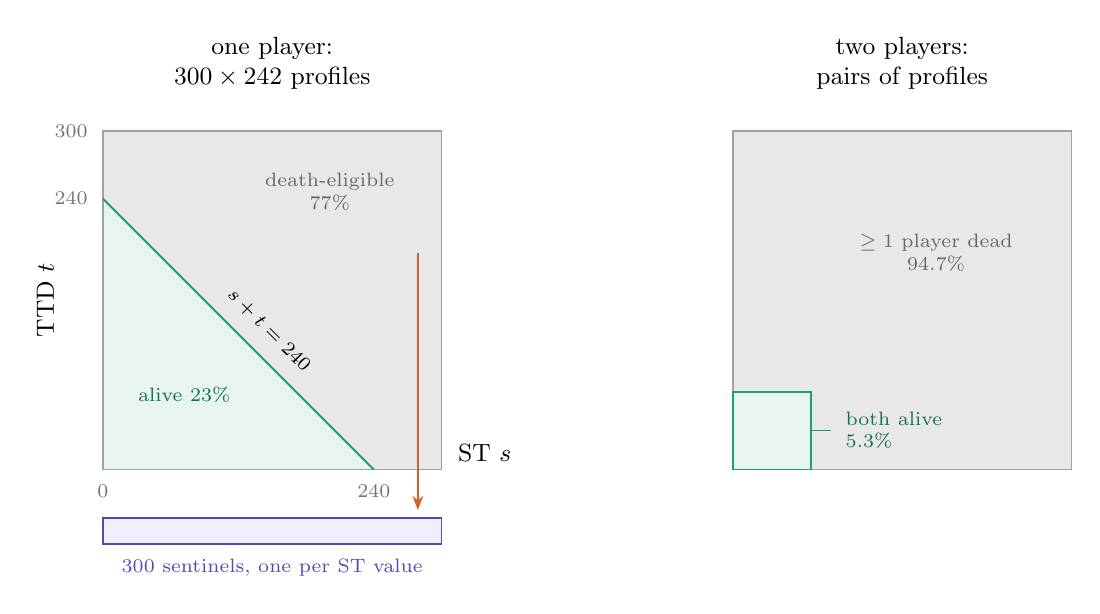
\begin{tikzpicture}[x=0.86cm, y=0.86cm]
% One-player profile geometry: the alive region is triangular, while every
% death-eligible vertical fibre collapses to one sentinel for its ST value.
\fill[figlightgray] (0,0) rectangle (5,5);
\fill[figpaleteal] (0,0) -- (4,0) -- (0,4) -- cycle;
\draw[figboxgray, line width=0.5pt] (0,0) rectangle (5,5);
\draw[figteal, line width=0.7pt] (4,0) -- (0,4);
\node[font=\scriptsize, rotate=-45] at (2.45,2.05) {$s+t=240$};
\node[font=\scriptsize, text=figteal!70!black] at (1.2,1.1)
  {alive $23\%$};
\node[font=\scriptsize, align=center, text=figink!70] at (3.35,4.1)
  {death-eligible\\$77\%$};
\fill[figpalepurple] (0,-1.1) rectangle (5,-0.72);
\draw[figpurple, line width=0.6pt]
  (0,-1.1) rectangle (5,-0.72);
\draw[-{Stealth[length=1.8mm]}, figorange, line width=0.8pt]
  (4.65,3.2) -- (4.65,-0.6);
\node[font=\scriptsize, text=figpurple, anchor=north] at (2.5,-1.18)
  {$300$ sentinels, one per ST value};
\node[font=\scriptsize, text=black!55, anchor=north] at (0,-0.08) {$0$};
\node[font=\scriptsize, text=black!55, anchor=north] at (4,-0.08) {$240$};
\node[font=\scriptsize, text=black!55, anchor=east] at (-0.08,4) {$240$};
\node[font=\scriptsize, text=black!55, anchor=east] at (-0.08,5) {$300$};
\node[font=\small, anchor=west] at (5.1,0.25) {ST $s$};
\node[font=\small, rotate=90] at (-0.85,2.5) {TTD $t$};
\node[font=\small, align=center] at (2.5,6.0)
  {one player:\\ $300\times242$ profiles};

% Two-player product geometry: the small square is the only region on which
% neither player's profile is quotiented.
\begin{scope}[xshift=8cm]
\fill[figlightgray] (0,0) rectangle (5,5);
\fill[figpaleteal] (0,0) rectangle (1.15,1.15);
\draw[figboxgray, line width=0.5pt] (0,0) rectangle (5,5);
\draw[figteal, line width=0.7pt] (0,0) rectangle (1.15,1.15);
\node[font=\scriptsize, align=center, text=figink!70] at (3.0,3.2)
  {$\geq 1$ player dead\\$94.7\%$};
\draw[figteal, line width=0.6pt] (1.15,0.575) -- (1.45,0.575);
\node[font=\scriptsize, align=left, text=figteal!70!black, anchor=west]
  at (1.52,0.575) {both alive\\$5.3\%$};
\node[font=\small, align=center] at (2.5,6.0)
  {two players:\\ pairs of profiles};
\end{scope}
\end{tikzpicture}
\caption{The quotient for one player (left) and for pairs of players
(right). Each vertical fibre in the death-eligible region collapses to one
sentinel per ST value. The left panel is schematic because TTD values
$1,\dots,59$ are unreachable (Lemma~\ref{lem:closure}); the percentages report
exact discrete counts on the transition-closed domain. The compact labels
``death-eligible'' and ``dead'' mean failure-fatal; neither means that a
player has already left the game.}
\label{fig:quotient}
\end{figure}

\section{The potential and the sweep schedule}\label{sec:potential}

The potential is not payoff, value, or strategic advantage. It is only a
progress score used to order the states.

\begin{definition}[Potential]\label{def:potential}
For a profile let $\rho(s,t)=t$ if $(s,t)$ is revival-eligible and
$\rho(s,t)=301$ otherwise; for a class let
\[
\Phi(x)=s_c+s_d+\rho(s_c,t_c)+\rho(s_d,t_d)\in\{0,\dots,1200\}.
\]
\end{definition}

\begin{theorem}[Strict increase]\label{thm:potential}
Every live transition strictly increases $\Phi$. By cases on the moving
profile:
\begin{itemize}[leftmargin=*]
\item successful lag $\ell$, the profile stays on the same side of the
  revival boundary:
  $\Delta\Phi=\ell\ge1$;
\item successful lag $\ell$, the profile becomes failure-fatal:
  $\Delta\Phi=\ell+301-t\ge\ell+61$, since revival-eligibility implies
  $t\le240$;
\item failure, revived profile remains revival-eligible: $\Delta\Phi=60$ (the ST resets to
  zero while TTD absorbs the dose);
\item failure, revived profile becomes failure-fatal:
  $\Delta\Phi=301-(s_c+t_c)\ge61$ by
  \eqref{eq:survive}.
\end{itemize}
\end{theorem}

\begin{corollary}[Layered backward induction]\label{cor:layers}
No transition stays within a $\Phi$-layer, so a descending sweep solves every
child before its parents. Any layer-$P$ residual work need only complete
before layer $P-1$ begins. The
$289{,}374{,}121$ classes occupy all $1{,}201$ layers; the largest,
$\Phi=374$, holds $1{,}678{,}715$ classes. Define the one-player bucket
\[
B_a=\{(s,t)\text{ quotient profiles}:s+\rho(s,t)=a\}.
\]
Then layer $P$ is exactly
\[
\Phi^{-1}(P)=
\bigcup_{\substack{0\le a\le600\\0\le P-a\le600}}B_a\times B_{P-a}.
\]
\end{corollary}

The quotient classes therefore form the layered DAG in
Figure~\ref{fig:potential-dag}.

\begin{figure}[H]
\centering
\begin{tikzpicture}[
  x=1cm,
  y=1cm,
  state/.style={circle, draw=figblue, fill=white, line width=0.7pt,
    minimum size=6mm, inner sep=0pt},
  focus/.style={state, draw=figteal, fill=figpaleteal, line width=0.9pt},
  edge/.style={-{Stealth[length=1.7mm]}, draw=figblue!75!black,
    line width=0.65pt},
  rank/.style={draw=figlightgray, dashed, line width=0.55pt},
]
\begin{scope}[yshift=2.85cm, yscale=0.72]
% Ranks are potential layers.
\draw[rank] (1.2,0.55) -- (1.2,3.75);
\draw[rank] (4.5,0.55) -- (4.5,3.75);
\draw[rank] (7.8,0.55) -- (7.8,3.75);
\draw[rank] (11.1,0.55) -- (11.1,3.75);
\node[font=\small] at (1.2,4.35) {$\Phi=P$};
\node[font=\small] at (4.5,4.35) {$\Phi=P+a$};
\node[font=\small] at (7.8,4.35) {$\Phi=P+b$};
\node[font=\small] at (11.1,4.35) {$\Phi=P+c$};

% A small representative subgraph. Some edges skip ranks, as transitions may
% increase the potential by more than one.
\node[state] (a1) at (1.2,1.00) {};
\node[focus] (a2) at (1.2,2.20) {$x$};
\node[state] (a3) at (1.2,3.40) {};

\node[state] (b1) at (4.5,0.80) {};
\node[state] (b2) at (4.5,1.70) {};
\node[state] (b3) at (4.5,2.70) {};
\node[state] (b4) at (4.5,3.60) {};

\node[state] (c1) at (7.8,1.00) {};
\node[state] (c2) at (7.8,2.20) {};
\node[state] (c3) at (7.8,3.40) {};

\node[state] (d1) at (11.1,1.35) {};
\node[state] (d2) at (11.1,3.05) {};

\draw[edge] (a1) -- (b1);
\draw[edge] (a1) -- (b2);
\draw[edge] (a2) -- (b2);
\draw[edge] (a2) -- (b3);
\draw[edge] (a2) -- (c2);
\draw[edge] (a3) -- (b3);
\draw[edge] (a3) -- (b4);
\draw[edge] (b1) -- (c1);
\draw[edge] (b2) -- (c1);
\draw[edge] (b2) -- (c2);
\draw[edge] (b3) -- (c2);
\draw[edge] (b3) -- (c3);
\draw[edge] (b4) -- (c3);
\draw[edge] (c1) -- (d1);
\draw[edge] (c2) -- (d1);
\draw[edge] (c2) -- (d2);
\draw[edge] (c3) -- (d2);

\draw[-{Stealth[length=2mm]}, draw=figpurple, line width=0.95pt]
  (11.1,0.10) -- (1.2,0.10);
\node[font=\scriptsize, text=figpurple, fill=white, inner sep=2pt]
  at (6.15,0.10) {backward solve};
\end{scope}

\begin{axis}[
  at={(0cm,0cm)}, anchor=south west,
  width=12.25cm, height=2.15cm,
  scale only axis,
  xmin=0, xmax=1200, ymin=0, ymax=1900000,
  axis lines=left,
  xlabel={potential layer $\Phi$},
  ylabel={classes},
  xtick={0,300,600,900,1200},
  ytick={0,800000,1600000},
  yticklabels={0,$0.8$M,$1.6$M},
  scaled y ticks=false,
  label style={font=\scriptsize},
  tick label style={font=\scriptsize},
  grid=major,
  grid style={draw=figlightgray, line width=0.4pt},
  clip=false,
]
\addplot[draw=figblue, fill=figblue!14, line width=0.75pt]
  table[x=potential, y=classes] {build/figures/layer_widths.dat}
  \closedcycle;
\addplot[only marks, mark=*, mark size=1.7pt, figorange]
  coordinates {(374,1678715)};
\node[anchor=south west, font=\scriptsize, text=figorange]
  at (axis cs:374,1678715) {peak: $1.68$M};
\end{axis}
\end{tikzpicture}
\caption{Top: representative transitions in the potential-ranked DAG.
Bottom: the exact linear-scale width of all $1{,}201$ layers. Every edge
points right; the computation runs from right to left.}
\label{fig:potential-dag}
\end{figure}

The strict increase was checked over all $1{,}035{,}541$ live profile
transitions. The schedule needs no reachability analysis, frontier queue, or
transposition table; it simply solves unreachable classes as well.

\section{Certified equilibria}\label{sec:certified}

\begin{definition}[Certificate]\label{def:certificate}
For a stage matrix $M$ and mixed strategies $\sigma_d$ (Dropper) and $\sigma_c$
(Checker), let
\[
L=\min_c(\sigma_d^{\mathsf T}M)_c,\qquad
U=\max_d(M\sigma_c)_d,\qquad
\gap_M(\sigma_d, \sigma_c)=\max(0,\,U-L).
\]
The pair \emph{certifies} the value $\widehat v=(L+U)/2$ at tolerance
$\tol$ when $\gap_M(\sigma_d,\sigma_c)\le\tol$. Throughout, $\tol=10^{-6}$, and
the gap is always measured against the \emph{full} matrix
\eqref{eq:toeplitz}.
\end{definition}

For example, $L=0.0898$ and $U=0.0899$ place the matrix value inside that
interval. The gap is $0.0001$; it measures how much room remains between the
two players' guarantees.

\begin{proposition}[Certified midpoint]\label{prop:midpoint}
$L\le\val(M)\le U$, so a certificate at tolerance $\tol$ pins
$|\widehat v-\val(M)|\le\tol/2$.
\end{proposition}

\begin{proof}
$\sigma_d$ guarantees the row player at least $L$ against every reply, and
$\sigma_c$ caps the row player at $U$; $\val(M)$ sits between the two
levels.
\end{proof}

\begin{lemma}[Matrix-value Lipschitz bound]\label{lem:lipschitz}
If $\max_{d,c}|M_{d,c}-\widehat M_{d,c}|\le\epsilon$, then
$|\val(M)-\val(\widehat M)|\le\epsilon$, since
$|\sigma_d^{\mathsf T}(M-\widehat M)\sigma_c|\le\epsilon$ for all mixed pairs.
\end{lemma}

\subsection{The solver ladder}

The support of a mixed strategy is the set of actions it uses with positive
probability:
\[
\operatorname{supp}(\sigma)=\{i:\sigma_i>0\}.
\]
Each class then follows the same three-step ladder.

\begin{enumerate}[leftmargin=*]
\item \textbf{Pure saddle.} Lemma~\ref{lem:toeplitz} computes the maximin
  and minimax in $O(60)$. If they meet, a deterministic action pair suffices.
\item \textbf{Equalizer.} A support guess reduces the mixed game to one
  linear system. A nearby solved support is tried first, then all sixty
  actions. Every candidate is checked against the full matrix.
\item \textbf{Linear programming.} The remaining matrices use the standard
  zero-sum primal and dual programs, followed by the same full-matrix check.
\end{enumerate}

The equalizer systems, support rule, and LPs are stated in
Appendix~\ref{sec:details}.

\subsection{Propagated error}

The table stores certified midpoints, so a parent's matrix is assembled
from child values that are themselves within a bounded distance of truth.

\begin{proposition}[A priori accumulated bound]\label{prop:accumulated}
Let every stored value carry a certificate at tolerance $\tol$ and let
$\delta(x)$ bound the longest live path from $x$ to a terminal. Then the
stored value $\widehat V(x)$ satisfies
\[
|\widehat V(x)-V(x)|\;\le\;\delta(x)\,\frac{\tol}{2}
\;\le\;\frac{1201-\Phi(x)}{2}\,\tol .
\]
In particular the initial state obeys
$|\widehat V-V|(0,0,0,0)\le6.1\times10^{-4}$.
\end{proposition}

\begin{proof}
Induction up the DAG. Terminal entries are exact. If every child satisfies
the bound with $\delta(x)-1$, the assembled matrix is entrywise within
$(\delta(x)-1)\tol/2$ of the true one (expectations and negation are
non-expansive), Lemma~\ref{lem:lipschitz} transfers that to the value, and
Proposition~\ref{prop:midpoint} adds the state's own $\tol/2$. Each
live-to-live transition raises $\Phi$ by at least one
(Theorem~\ref{thm:potential}), so a play from $x$ makes at most
$1200-\Phi(x)$ of them plus one terminal transition, bounding $\delta$.
\end{proof}

\subsection{Policy certification}

At each live class $x$, let
$(\widehat\sigma_d(x),\widehat\sigma_c(x))$ be the accepted mixed pair.
Using that pair whenever $x$ is reached defines a behavioral policy
$\widehat\pi$. A deviation may replace every remaining choice, not only the
next action.

\begin{definition}[Policy security values]\label{def:policy-gap}
For two complete policies, extend the value notation by
\[
V_x(\pi_d,\pi_c)
=\mathbb E[\text{terminal payoff}\mid x,\pi_d,\pi_c].
\]
The subscripts $d,c$ identify the players by their roles at $x$; both policies
include play after later role swaps. The selected policies have security
values
\begin{align*}
\underline V_{\widehat\pi}(x)
&=\min_{\pi_c}
  V_x(\widehat\pi_d,\pi_c),\\
\overline V_{\widehat\pi}(x)
&=\max_{\pi_d}
  V_x(\pi_d,\widehat\pi_c).
\end{align*}
\end{definition}

The policy's own payoff lies between these values:
\[
\underline V_{\widehat\pi}(x)
\le V_x(\widehat\pi_d,\widehat\pi_c)
\le\overline V_{\widehat\pi}(x).
\]
Hence either player's gain from a unilateral deviation is bounded by
$\overline V_{\widehat\pi}(x)-\underline V_{\widehat\pi}(x)$.

Let $\varepsilon(x)$ be the largest sum of accepted matrix gaps along any
continuation from $x$ to a terminal state. For a live state $x$, let $y$ be a
live child of $x$. Then
\begin{equation}\label{eq:policy-epsilon}
\varepsilon(x)=
\begin{cases}
0, & x\text{ terminal},\\[2pt]
(U_x-L_x)
+\displaystyle\max_y
 \varepsilon(y), & x\text{ live}.
\end{cases}
\end{equation}
The maximum is zero when $x$ has no live child.

\begin{proposition}[Full-policy bound]\label{prop:policy}
The selected policy satisfies
\begin{align*}
\underline V_{\widehat\pi}(x)
&\ge \widehat V(x)-\tfrac12\varepsilon(x),\\
\overline V_{\widehat\pi}(x)
&\le \widehat V(x)+\tfrac12\varepsilon(x).
\end{align*}
Consequently,
\[
\overline V_{\widehat\pi}(x)-\underline V_{\widehat\pi}(x)
\le \varepsilon(x)
\le (1201-\Phi(x))\tol.
\]
At the initial state, the payoff gap is at most
$1.201\times10^{-3}$, so no unilateral deviation can improve win probability
by more than $6.005\times10^{-4}$.
\end{proposition}

\begin{samepage}
\begin{proof}
At a terminal,
$\underline V_{\widehat\pi}
=\overline V_{\widehat\pi}=\widehat V$ and $\varepsilon=0$.
Suppose the two bounds hold for every live child of $x$. Negation at a role
swap and averaging after revival preserve the largest child bound. Therefore
\begin{align*}
\underline V_{\widehat\pi}(x)
&\ge L_x-\tfrac12
  \max_y\varepsilon(y),\\
\overline V_{\widehat\pi}(x)
&\le U_x+\tfrac12
  \max_y\varepsilon(y).
\end{align*}
Since $\widehat V(x)=(L_x+U_x)/2$, recurrence
\eqref{eq:policy-epsilon} gives the two stated bounds.

Finally, $U_x-L_x\le\tol$ at every live state, and every continuing transition
raises $\Phi$ by at least one. Hence no path from $x$ contains more than
$1201-\Phi(x)$ live states.
\end{proof}
\end{samepage}

\section{The computation}\label{sec:computation}

\subsection{Sweep schedule}

The potential turns the computation into a fixed order rather than a search.
The solver starts at $\Phi=1200$ and moves left across Figure~\ref{fig:potential-dag}
to $\Phi=0$; within a layer, its bucket rectangles are independent and can run
in parallel. Revival probabilities are evaluated once, and each completed
layer is checkpointed before the next begins.

\subsection{Results}

The sweep covered all $289{,}374{,}121$ classes across checkpointed
sessions on a single twelve-core consumer desktop (AMD Ryzen~9 3900X). The
final session --- $283{,}764{,}990$ classes, $98.1\%$ of the table ---
completed in $5{,}432$ seconds ($1.51$ hours); the remaining
$5{,}609{,}131$ classes were built in earlier, untimed sessions. The
previously recorded single-core projection for the unquotiented,
search-based design was $3.7$--$5.1$ years; that ratio mixes three
factors: the $18.2\times$ quotient, the sweep-for-search redesign, and
twelve-way parallelism.

The solver routes show which optimizations actually mattered:

\begin{center}
\begin{tabular}{@{}lrr@{}}
\toprule
rung & classes & share\\
\midrule
pure saddle (Lemma~\ref{lem:toeplitz}) & $334{,}588$ & $0.116\%$\\
equalizer, warm-started support & $38{,}138$ & $0.013\%$\\
equalizer, full support ($k=60$) & $288{,}810{,}400$ & $99.805\%$\\
linear programming & $190{,}995$ & $0.066\%$\\
\bottomrule
\end{tabular}
\end{center}

\noindent
The full-support equalizer did almost all of the work. The warm solver rarely
helped because its twelve-action cap could not represent the mostly
full-support equilibria; linear programming was still needed for the final
$0.066\%$ of classes.

\begin{figure}[H]
\centering
\begin{tikzpicture}
\begin{axis}[
  width=0.95\textwidth, height=5.8cm,
  xlabel={second}, ylabel={probability},
  xmin=0, xmax=61, ymin=0.005, ymax=0.35,
  ymode=log,
  log ticks with fixed point,
  ytick={0.005,0.01,0.03,0.1,0.3},
  yticklabel style={/pgf/number format/fixed},
  legend style={at={(0.5,0.97)}, anchor=north, legend columns=2},
]
\addplot[figblue, line width=0.8pt, mark=*, mark size=1pt]
  table[x=action, y=drop] {build/figures/root_strategies.dat};
\addplot[figorange, dashed, line width=0.8pt, mark=*, mark size=1pt]
  table[x=action, y=check] {build/figures/root_strategies.dat};
\legend{Dropper $\sigma_d$, Checker $\sigma_c$}
\end{axis}
\end{tikzpicture}
\caption{The first-round strategies of the selected full-game policy. Their
local gap is $3.2\times10^{-15}$; Proposition~\ref{prop:policy} shows how
later gaps accumulate. Both strategies have full support.}
\label{fig:root}
\end{figure}

The Python and Rust sweeps agreed byte-for-byte on their overlapping regions;
$4{,}792$ sampled Bellman re-solves differed by at most
$4.84\times10^{-7}$. The error bound itself is
Proposition~\ref{prop:accumulated}.

\begin{theorem}[Main result]\label{thm:main}
The complete 60-action timing model of Section~\ref{sec:game} has a certified
numerical solution on the transition-closed quotient domain of
Lemma~\ref{lem:closure}. Every one of its $289{,}374{,}121$ classes carries a
stored midpoint with local gap at most $10^{-6}$. At the initial state,
\[
V(0,0,0,0)=0.08985\pm0.00061,
\qquad
P(\text{first Dropper wins})=0.54493\pm0.00031.
\]
For the selected full-game policy,
\[
\overline V_{\widehat\pi}(0,0,0,0)
-\underline V_{\widehat\pi}(0,0,0,0)
\le1.201\times10^{-3}.
\]
\end{theorem}

\FloatBarrier
\section{Scope of the claims}\label{sec:claims}

\begin{itemize}[leftmargin=*]
\item \textbf{Rules-relative.} The results concern Section~\ref{sec:game} and
  the frozen revival surface \eqref{eq:revival}, not the leap-aware game with
  its asymmetric 61st second.
\item \textbf{Certified numerics.} Values are round-to-nearest float64
  midpoints with saddle-gap certificates, not rational or interval
  arithmetic. The structural theorems are exact; survival, absorption,
  counting, and potential increase were exhaustively enumerated.
\item \textbf{Domain.} The table covers the transition-closed quotient
  domain; states containing a revival-eligible profile with TTD in $1..59$
  are outside it and are rejected, not approximated
  (Lemma~\ref{lem:closure}).
\item \textbf{Policies.} The table stores values and routing; accepted
  strategies are re-derived from child values. Figure~\ref{fig:root} shows
  the first pair.
\end{itemize}

\appendix
\begin{samepage}
\section{Computational details}\label{sec:details}

\subsection{Sweep}

One-player quotient profiles are indexed by $p\in\{0,\dots,17{,}010\}$; a
state class is stored at $17{,}011p_c+p_d$. For
$P=1200,1199,\dots,0$, the solver:

\begin{enumerate}[leftmargin=*]
\item enumerates the rectangles $B_a\times B_{P-a}$;
\item builds $S_1,\dots,S_{60}$ and $F$ from already solved children;
\item tries the pure, equalizer, and LP rungs in order;
\item recomputes $L$ and $U$ against the full matrix and stores their midpoint
  only when $U-L\le\tol$;
\item checkpoints the completed layer before moving to $P-1$.
\end{enumerate}

Revival probabilities are evaluated once. Classes within one layer are
independent.
\end{samepage}

\subsection{Equalizer and LP fallbacks}

Warm supports come from $(T_1p_c,p_d)$ and $(p_c,T_1p_d)$, where $T_1$ adds
one second of ST and applies the quotient. Masses at most $10^{-9}$ are
removed and each support is capped at its twelve largest actions. Let
$k=\min(|D|,|C|)$; the first $k$ actions in each support give
\[
\begin{pmatrix}M_{D,C}&-\mathbf 1\\ \mathbf 1^{\mathsf T}&0\end{pmatrix}
\begin{pmatrix}\sigma_{c,C}\\ u_c\end{pmatrix}
=\begin{pmatrix}\mathbf 0\\ 1\end{pmatrix},
\qquad
\begin{pmatrix}M_{D,C}^{\mathsf T}&-\mathbf 1\\
\mathbf 1^{\mathsf T}&0\end{pmatrix}
\begin{pmatrix}\sigma_{d,D}\\ u_d\end{pmatrix}
=\begin{pmatrix}\mathbf 0\\ 1\end{pmatrix}.
\]
A pivot below $10^{-12}$ or mass below $-10^{-12}$ rejects the candidate.
The full-support attempt uses $D=C=\{1,\dots,60\}$.

The residue is solved by the standard zero-sum pair
\[
\begin{aligned}
\max_{\sigma_d,v}\quad &v
&&\text{s.t.}\quad M^{\mathsf T}\sigma_d\ge v\mathbf1,\quad
\mathbf1^{\mathsf T}\sigma_d=1,\quad\sigma_d\ge0,\\
\min_{\sigma_c,u}\quad &u
&&\text{s.t.}\quad M\sigma_c\le u\mathbf1,\quad
\mathbf1^{\mathsf T}\sigma_c=1,\quad\sigma_c\ge0.
\end{aligned}
\]

\section{Reproducibility}

From the repository root, \texttt{uv run python -m dth complete} builds the
checkpointed artifact with
\texttt{src/dth/config/complete\_full\_v1.yaml}; its stored root midpoint is
\texttt{0.0898500728095116}.

\vspace{-0.8em}
\begin{thebibliography}{9}
\footnotesize
\setlength{\itemsep}{0pt}

\bibitem{stlevidence}
Toshio Sako. \emph{Usogui}. Shueisha, 2006--2018.
\newblock Source evidence indexed in \emph{Canonical game evidence}, project
ledger entries E-CYLINDER-CAP, E-DOSE-COMPOSITION, E-PROXIMITY-RISK,
and E-TTD-SLACK, 2026.
\newblock \href{https://youngjump.jp/manga/usogui/}{Official series page.}

\bibitem{zermelo1913}
Ernst Zermelo.
\newblock \"Uber eine Anwendung der Mengenlehre auf die Theorie des
Schachspiels.
\newblock In \emph{Proceedings of the Fifth International Congress of
Mathematicians}, volume 2, pages 501--504, Cambridge, 1913.

\bibitem{vonneumann1928}
John von Neumann.
\newblock Zur Theorie der Gesellschaftsspiele.
\newblock \emph{Mathematische Annalen}, 100:295--320, 1928.
\newblock \href{https://doi.org/10.1007/BF01448847}{doi:10.1007/BF01448847}

\bibitem{shapley1953}
Lloyd S. Shapley.
\newblock Stochastic games.
\newblock \emph{Proceedings of the National Academy of Sciences},
39(10):1095--1100, 1953.
\newblock \href{https://doi.org/10.1073/pnas.39.10.1095}%
{doi:10.1073/pnas.39.10.1095}

\end{thebibliography}

\end{document}
